\chapter{Arquitectura del sistema}  \label{arquitectura_sec}
\section{Flujo de trabajo}  \label{workflow_subsecc}

Describiremos el diseño confeccionado en detalle. Se tienen tres etapas fundamentales:

\begin{itemize}
\item \textbf{Pre-procesamiento:} consiste en capturar la imagen aplicando las
  transformaciones mencionadas en la sección \ref{dynamicrange} y
  \ref{fixedpoint}, empleando un script hecho en Python. Este script divide la
  imagen en lotes o batches y los envía a la FPGA, a través del puerto UART. Un
  batch o lote, consiste en columnas contiguas de pixeles cuya dimensión se
  explica en la sección~\ref{storage_subsecc}.
\item \textbf{Procesamiento:}	: el batch es convolucionado con el kernel dentro del módulo. Dicho kernel es configurable, y el usuario puede cargar los coeficientes del mismo mediante el GPIO. 
  Cuando la operación de la convolucion finaliza, una notificación es enviada a
  un microprocesador en la FPGA, que da la orden de recuperar el batch procesado, para así enviarlo a la unidad central de procesamiento (CPU).
\item \textbf{Post-procesamiento:}Como etapa final, en el post-procesamiento se combinan los batches o lotes en CPU usando el script de Python.
\end{itemize}

\section{Estados y transiciones}  \label{states_subsecc}

\begin{figure}
\centering
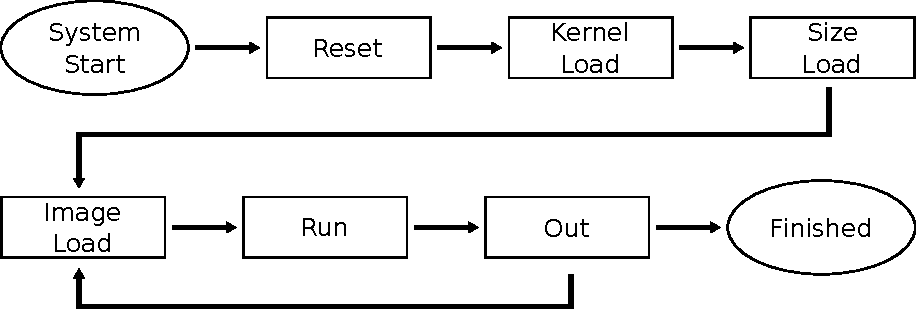
\includegraphics[scale=0.7]{states.pdf}
\caption{Diagrama de estados del sistema.}
\label{statesfig}
\end{figure}

El módulo atraviesa distintos estados para llevar a cabo su tarea. Estos estados
se pueden observar en la figura~\ref{statesfig}.

La transición entre un estado y
otro se realiza mediante instrucciones codificadas en el frame de entrada de 32
bits asentado en el GPIO. El módulo permanece en su estado actual hasta recibir
una instrucción valida.

Inicialmente, debe situarse al sistema en un estado de reset, y por ende debe
recibir una señal de reset para establecerse en dicho estado, esperando a ser
configurado.
Luego de recibir la correspondiente instrucción, se produce una transición hacia el estado KernelLoad, en donde los coeficientes del kernel se cargan al módulo.
El siguiente estado (SizeLoad), es en el cual se carga el tamaño de la imagen,
más precisamente la altura de la misma, esto permitirá conocer la posición del
último dato en memoria.
Estos tres estados mencionados, solo se ejecutan una vez durante todo el ciclo
de trabajo. El proceso se repite por cada nueva imagen, por ende, si se desea
procesar una nueva imagen, inicia el ciclo nuevamente.

Pasada la etapa de carga, la primera transición es hacia el
estado ImageLoad, donde se almacena el lote en la Block RAM de la FPGA.
Teniendo el lote almacenado, la transición luego es hacia el estado run donde se
hace el filtrado del lote, y mientras el sistema se situe en este estado, no
puede ser interrumpido.
Como consecuencia, cualquier instrucción recibida se ignora hasta que se
complete esta etapa de procesamiento de lote.

Cuando se finaliza el procesamiento de un lote, se emite una notificación y el sistema
queda en espera de la última señal para pasar hacia el estado Out. Una vez recibida la
correspondiente instrucción codificada, se devuelve el lote procesado al
microprocesador de la PC.

\begin{figure}
\centering
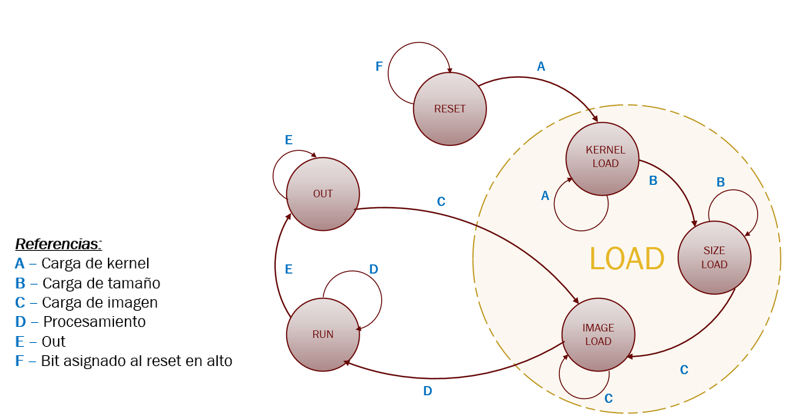
\includegraphics[scale=0.7]{states_2.png}
\caption{Diferentes estados y las etapas involucradas }
\label{statesfig2}
\end{figure}

\section{Arquitectura del módulo de convolución}  \label{ourdesign_subsecs}

El diseño planteado prioriza la reutilización dinámica de memoria, en donde por
cada iteración en la etapa de procesamiento, se aprovecha la disponibilidad de
datos cargados en memoria en la iteración anterior.
En la figura~\ref{general}, se muestran los bloques principales que conforman el
diseño. Los bloques que integran el módulo son:

\begin{figure}
\centering
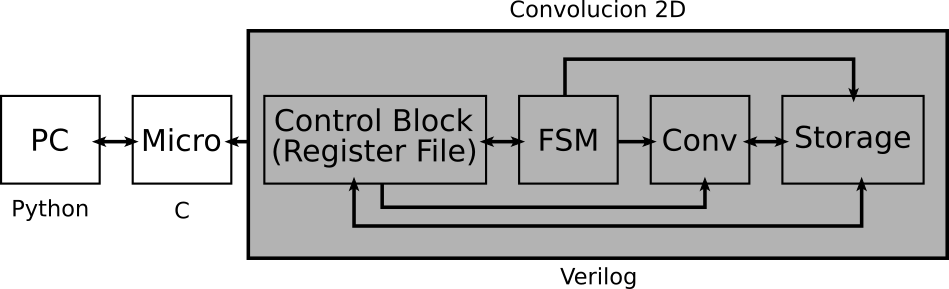
\includegraphics{general}
\caption{Arquitectura general del sistema }
\label{general}
\end{figure}

\begin{itemize}
\item \textbf{Control Unit:} se encarga del manejo de la comunicación entre el
  módulo y el procesador instanciado en la FPGA.\@
\item \textbf{MAC Unit -Multiplier-ACcumulator:} ejecuta la suma de los productos entre los coeficientes del kernel y los pixeles de la imagen. 
\item \textbf{Address Generation Unit (AGU):} bloque que maneja las direcciones
  de memoria que deben ser leídas o escritas.
\item \textbf{Memory Management Unit (MMU):} decide como son escritos y leídos
  los datos en la memoria.
\item \textbf{Storage:} hace referencia a un conjunto de columnas formadas por
  BRAMs de la FPGA.\@ El tamaño depende de la cantidad de MACs instanciadas,
  o en otras palabras, el paralelismo a nivel de cantidad de convoluciones en
  paralelo, que se desee en el sistema.
\end{itemize}
     
Estos bloques se describen en mas detalle en las secciones siguientes.

\subsection{Storage}\label{storage_subsecc}

Para almacenar un lote, se opto por organizar la BRAM en
columnas. Cada columna entonces, corresponde a una columna del lote.

El tamaño del lote está dado por la altura de la imagen y por el número de
columnas de memoria instanciadas.  La máxima altura en pixels de la imagen,
entonces, debe ser menor o igual al número de direcciones de una columna de
memoria instanciada.

Durante el procesamiento del lote, cada pixel se lee únicamente una vez, lo que
permite un uso mas eficiente de la memoria. Los pixeles del lote que ya fueron
leídos, se sobrescriben con los pixeles procesados. Esto permite reducir la
cantidad de memoria necesaria, ya que reúsa la misma memoria para almacenar el
lote de entrada, y el lote procesado.

Estas columnas de BRAM poseen dos puertos de direcciones y datos, uno para
los datos de entrada y otro para los datos de salida y además una señal de
control, write enable, que habilita la escritura de los datos de entrada en la memoria.

\subsection{Control Unit}\label{sec:ctrl_u}
El bloque Control Unit es el encargado de hacer de interfaz entre los bloques
restantes del módulo de convolución y el microprocesador que se encuentra en la
FPGA.\@ Para hacer esto, cuenta con dos puertos de 32 bits conectados a los GPIO
de entrada y salida del procesador.

El bloque interpreta las instrucciones que recibe y modifica las señales de
control conectadas a los otros bloques, esto representa la transición de
estados mencionada en la sección~\ref{states_subsecc}.

La organización del frame de entrada de 32 bits, junto con los códigos binarios
de las instrucciones se muestra en la tabla~\ref{instr}.

\begin{table}
% increase table row spacing, adjust to taste
\renewcommand{\arraystretch}{1.3}
% if using array.sty, it might be a good idea to tweak the value of
% \extrarowheight as needed to properly center the text within the cells
\caption{Código de instrucciones, la letra ``d'' representa bit de datos.}\label{instr}
\centering
% some packages, such as mdw tools, offer better commands for making tables
% than the plain latex2e tabular which is used here.
\begin{tabular}{|l|c|c|c|c|c|}
  \hline
  \multicolumn{1}{|c|}{\multirow{2}{*}{\textbf{Instrucción}}} & \multicolumn{5}{c|}{\textbf{BITS}} \\ \cline{2-6}
                                        & \textbf{31 - 29} & \textbf{28 - 25} & \textbf{24 - 14} & \textbf{13 - 1} & \textbf{0}\\\hline
  Cargar kernel                         & 000              & xxx              & ddddddddddd      & ddddddddddddd   & 0         \\\hline
  Cargar tamaño imagen                  & 001              & xxx              & xxxxxxxxxxx      & xxxdddddddddd   & 0         \\\hline
  Cargar lote                           & 010              & xxx              & xxxxxxxxxxx      & ddddddddddddd   & 0         \\\hline
  Recuperar dato                        & 011              & xxx              & xxxxxxxxxxx      & xxxxxxxxxxxxx   & 0         \\\hline
  Finalización de lote                  & 100              & xxx              & xxxxxxxxxxx      & ddddddddddddd   & 0         \\\hline
\end{tabular}           
\end{table}

Como el módulo y el procesador trabajan a distintas frecuencias de reloj, se
puede producir un error al enviar y recibir datos entre ambos. Para superar este
problema, el flanco ascendente del bit 28 se utiliza como indicador de que un
nuevo dato esta listo para ser leído o escrito. 

El bit 0 se utiliza como indicador del estado del módulo, en caso de ser 1 el
módulo se pone en estado de reset, por lo que una vez atravesado este estado,
siempre debería permanecer bajo.

Las instrucciones cumplen las siguientes funciones:

\begin{itemize}
\item \textbf{Cargar kernel:} Se utiliza para cargar los coeficientes del
  kernel, cada coeficiente es de 8 bits, junto con la instrucción se deben
  añadir los 3 coeficientes que forman una fila del kernel.\footnote{Para un
    diseño que utiliza kernels de $3\times3$, en caso de ser de dimensiones
    superiores, nuevas instrucciones deben ser añadidas.}
\item \textbf{Cargar tamaño imagen:} A esta instrucción debe acompañar el tamaño
  del alto en pixels de la imagen, se utilizan 10 bits para ello por lo que el
  tamaño máximo es de 1024px.
\item \textbf{Cargar lote:} Instrucción que indica que los datos corresponden a
  un pixel del lote.
\item \textbf{Finalización de lote:} Indica que el pixel que se esta cargando es
  el último pixel del lote, una vez recibida esta instrucción el módulo pasa al
  estado de run donde realiza el procesamiento.
\item \textbf{Recuperar dato:} Con esta instrucción se pide al módulo que
  entregue el pixel procesado siguiente.
\end{itemize}

Como se nombró anteriormente, una instrucción no será considerada hasta que no
haya un flanco ascendente en el bit 28.

\subsection{Address Generator Unit (AGU)}

El AGU es el encargado de generar las direcciones de memoria que son
consumidas por el MMU.

Durante el estado de ImageLoad, el AGU genera las direcciones donde se deben
escribir estos datos, para ello cuenta con un contador que se incrementa con
cada flanco de subida del bit 28 de la entrada del Control Unit
(sección~\ref{sec:ctrl_u}). El AGU además conoce el alto de la imagen (cargado
durante SizeLoad) por lo que una vez que el contador alcanza dicho valor envía
una señal al MMU indicando que el pixel que se recibe a continuación pertenece a
una nueva columna del lote.

Durante la etapa de procesamiento el AGU debe producir dos direcciones
diferentes, una que indica al MMU los datos que debe entregar a las unidades MAC
y otra que indica al MMU la posición donde los datos procesados por las MACs
deben ser almacenados. Ambas direcciones se incrementan una vez por ciclo de
reloj, pues las MAC generan un dato procesado por ciclo. La diferencia entre la
dirección de lectura y la dirección de escritura es igual a la latencia que
existe desde que se entrega el primer pixel a una unidad MAC hasta que el primer
pixel procesado este listo para almacenarse.

Durante el estado Out, o de salida de datos, el AGU genera las direcciones de
lectura de los datos procesados, al igual que en el estado de ImageLoad, se
incrementa con cada flanco de subida del bit 28 y tiene en cuenta el alto de la
imagen para hacer el cambio de columna de datos.

\subsection{Multiplier Accumulator Unit (MAC)}\label{sec:MAC}

Las MACs son unidades que se instancian en paralelo, son las encargadas de
hacer el calculo necesario para realizar la convolución. Poseen 9 registros
donde se almacenan los coeficientes del kernel y 9 registros donde se almacenan
los pixels de la porción del lote que se esta procesando en ese instante.

Las MAC poseen un único puerto de entrada de datos, donde se ingresan 3
coeficientes (correspondientes a una fila) del kernel o de una sección de lote
según le sea indicado por una señal proveniente del Control Unit. Además se
tiene otra señal de control donde se indica si los registros deben ser
modificados o permanecer congelados.

Para un kernel de tamaño $(k \times k)$, cada MAC Unit toma $k$ columnas de memoria
adyacentes como entrada. Se cargan entonces k pixeles de cada columna, quedando
$(k \times k)$ pixeles cargados dentro de ella, lo necesario para producir el
primer pixel procesado. Luego, se procede a efectuar la multiplicación de los
pixeles con los coeficientes del kernel y sumar cada termino. Al finalizar la
suma de los productos, el rango de los datos aumenta, por lo que antes de
ponerlos a la salida, las MAC realizan un truncado sobre los resultados.

\begin{figure}
\centering
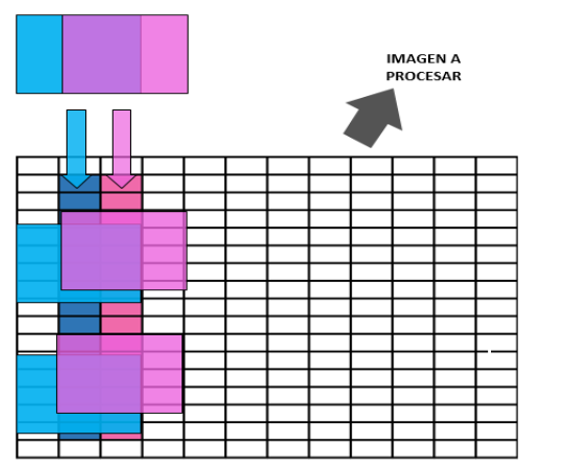
\includegraphics[scale=0.7]{conv1_despl.png}
\caption{Desplazamiento vertical del kernel sobre la imagen }
\label{verticaldesp}
\end{figure}

Una vez procesado un pixel, se efectua un desplazamiento (shift) de sus
registros en donde se almacenan pixeles del lote, para así descartar los $k$
pixeles mas antiguos, y se cargan los $k$ nuevos pixeles, es decir, una nueva
fila, lo que es equivalente a una estructura FIFO (First Input – First Output).
Se sincroniza lo mencionado anteriormente de forma tal de obtener un pixel
procesado por cada ciclo de reloj. Este procedimiento es equivalente a desplazar
verticalmente el kernel sobre la imagen como muestra la figura~\ref{verticaldesp}.

La estructura de hardware para realizar la operación se muestra en la figura~\ref{conv_struct},
como el hardware combinacional de los productos en cascada con la suma tiene un
tiempo de establecimiento de la salida mayor al período de reloj, se
introdujeron registros entre el hardware de los productos y la suma. Si bien
esto impacta en la latencia del bloque, la frecuencia de procesamiento se
mantiene en un pixel procesado por ciclo de reloj. 

\begin{figure}
\centering
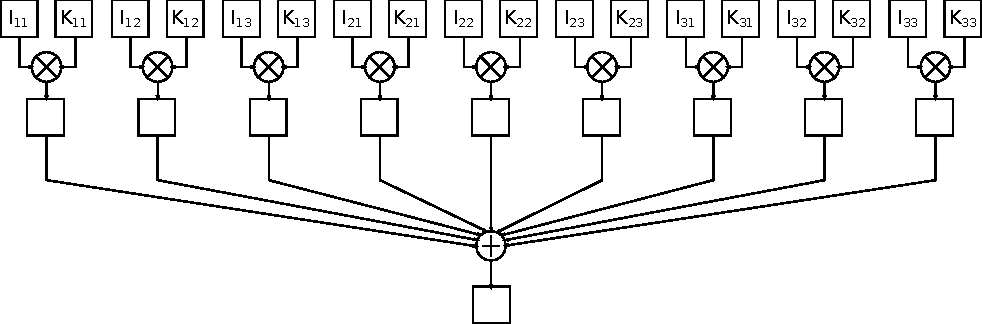
\includegraphics[scale=0.7]{conv_struct}
\caption{Estructura donde se realiza el calculo dentro de una unidad MAC.}
\label{conv_struct}
\end{figure}

\subsection{Memory Management Unit (MMU)}

Como se verá a continuación, para hacer un uso eficiente de las memorias es
necesario tener en cuenta el nivel de paralelismo. El objetivo del MMU es hacer
de interfaz entre las memorias y el resto de los bloques, independizándolos así del
nivel de paralelismo y reduciendo su complejidad.

En la sección~\ref{sec:MAC} se explicó que para un kernel de dimensión
$k \times k$ se necesitan $k$ columnas como entrada para producir una columna
procesada en una $MAC$ $Unit$. Por lo tanto, $2 \times k$ columnas, se necesitan
para $2$ $MACs$. Debido a la naturaleza de la operación de la convolución, para
obtener una columna contigua, se necesita desplazar una vez las columnas de
entrada. Entonces, existe un solapamiento entre las entradas de las MACs
que producen columnas adyacentes, y así la información puede ser compartida. 
Por esto, pese a necesitar $k$ columnas de entrada por cada unidad $MAC$,
solamente $k+1$ columnas diferentes de entrada se necesitan para dos $MACs$
instanciadas. Extendiendo este concepto a $N$ $MACs$, el número requerido de
columnas de memoria se reduce de $N \times k$ a $N+k-1$, concluyendo que
agregar una nueva unidad $MAC$ solamente agrega una nueva columna de memoria.

Debido al mismo solapamiento explicado anteriormente, hay información repetida entre
un lote recibido y el siguiente, por lo que, para reducir la transmisión de
datos, esta información repetida se mantiene en memoria y solamente se transmite
la parte faltante del lote entrante. Dadas $N$ $MACs$ y un kernel de $k \times k$,
un lote cuyo ancho (o cantidad de columnas) sea de $N+k-1$ es necesario. No
obstante, el lote procesado tendrá un ancho de  $N$ columnas, es decir, una por
unidad $MAC$, por lo que las ultimas $k+1$ memorias no se sobrescriben y
mantienen los datos de entrada. Estas $k+1$ columnas se reutilizan como las
primeras columnas del siguiente lote, y asi, el ancho del lote transmitido se
reduce a $N$, con la excepción de que el primer lote mantiene un ancho de
$N+k-1$.

La reutilización de columnas de memoria escritas por los lotes previos, resulta
en un desplazamiento circular en $N$ lugares, desplazando la posición de las
columnas de memoria asociadas con cada unidad $MAC$ en cada iteración. De lo
anterior, se deduce que existe una periodicidad entre la relación de columnas de
memoria y las entradas de las unidades $MAC$, donde el periodo $It$ es el número
de iteraciones necesario para obtener la relación ente las columnas de memoria
originales con respecto a las entradas de las unidades $MAC$. Matemáticamente
esto ocurre cuando $It$ es un múltiplo de $N+k-1$, esto es, debe existir un
número entero $m$, tal que:

\begin{equation}\label{niter}
  \frac{It}{m} = \frac{N}{k-1} + 1
\end{equation}

Comparado con un enfoque naive, donde cada MAC unit tendría sus $k$ columnas de
memoria independientes, el compartir información entre distintas MACs produce un
ahorro en el tamaño de BRAM necesaria, mientras que el desplazamiento circular
produce un ahorro en la cantidad de información transmitida. La
figura~\ref{comp} muestra una comparación de recursos utilizados por los
diferentes abordajes. Analizando la figura~\ref{transmitted} se observa que con el
abordaje naive es necesario transmitir casi 3 veces mas información (por ser un
kernel de $3 \times 3$) y no se ve afectado por el nivel de paralelismo.
En el caso de las entradas compartidas sin desplazamiento se tiene a disminuir
los datos redundantes transmitidos a medida que $N$ aumenta, esto es porque los
datos redundantes en un lote de $N+k-1$ es $k-1$ y $\frac{k-1}{N+k-1}$ tiende a
cero a medida que $N$ incrementa. El abordaje de las entradas compartidas con
desplazamiento circular es el caso óptimo donde no hay información redundante
transferida.

\begin{figure}%[!t]
\centering
\subfloat[][Cantidad de memoria requerida.]{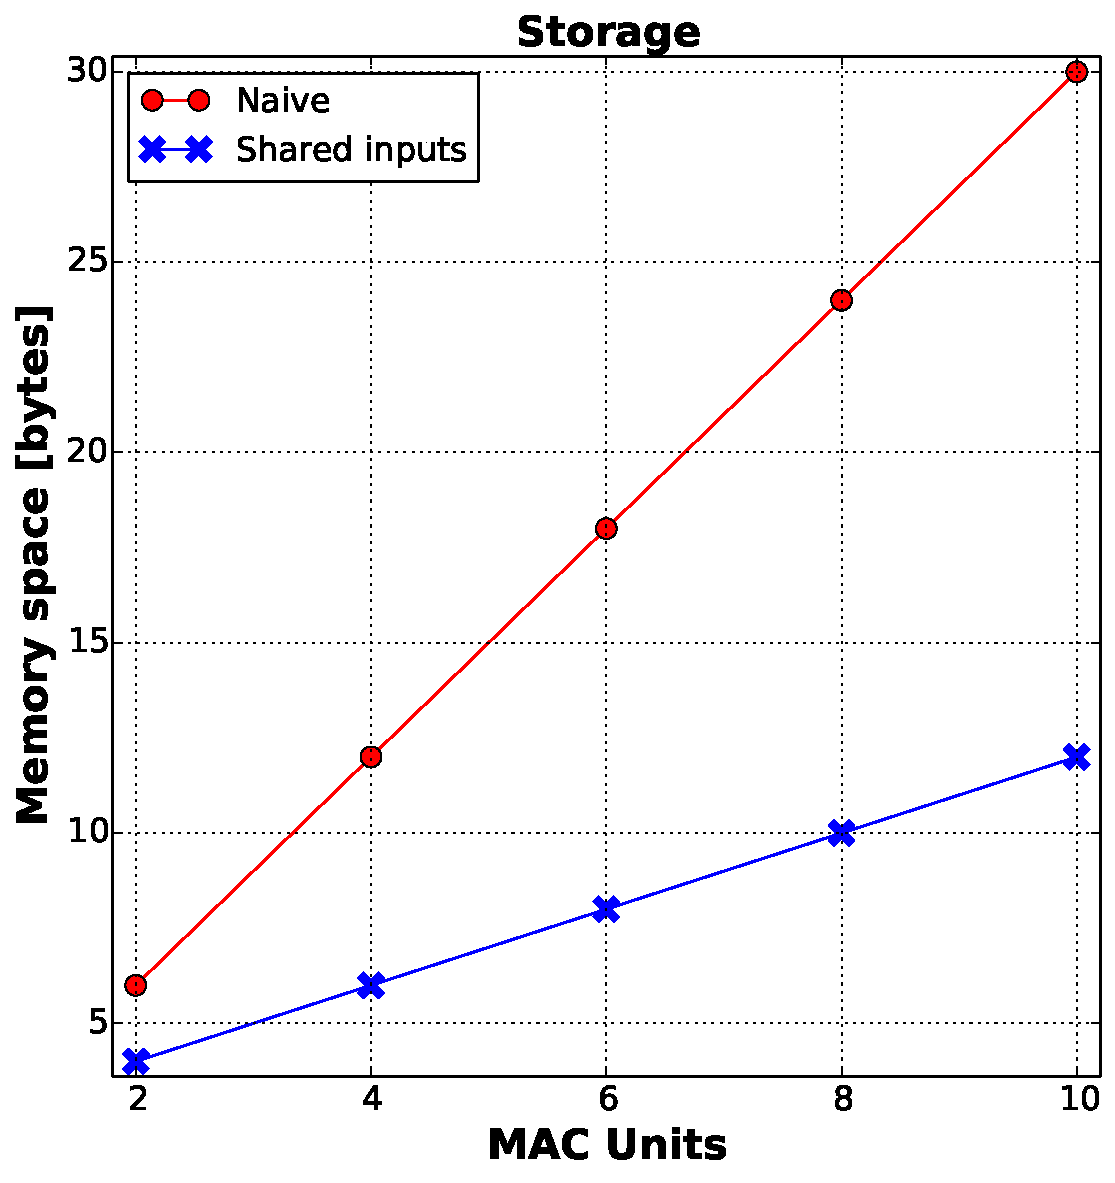
\includegraphics[scale=0.3]{mem_space2}%
\label{mem}}
\hfil %\vspace{0.1cm}
\centering
\subfloat[][Cantidad de datos transmitidos ]{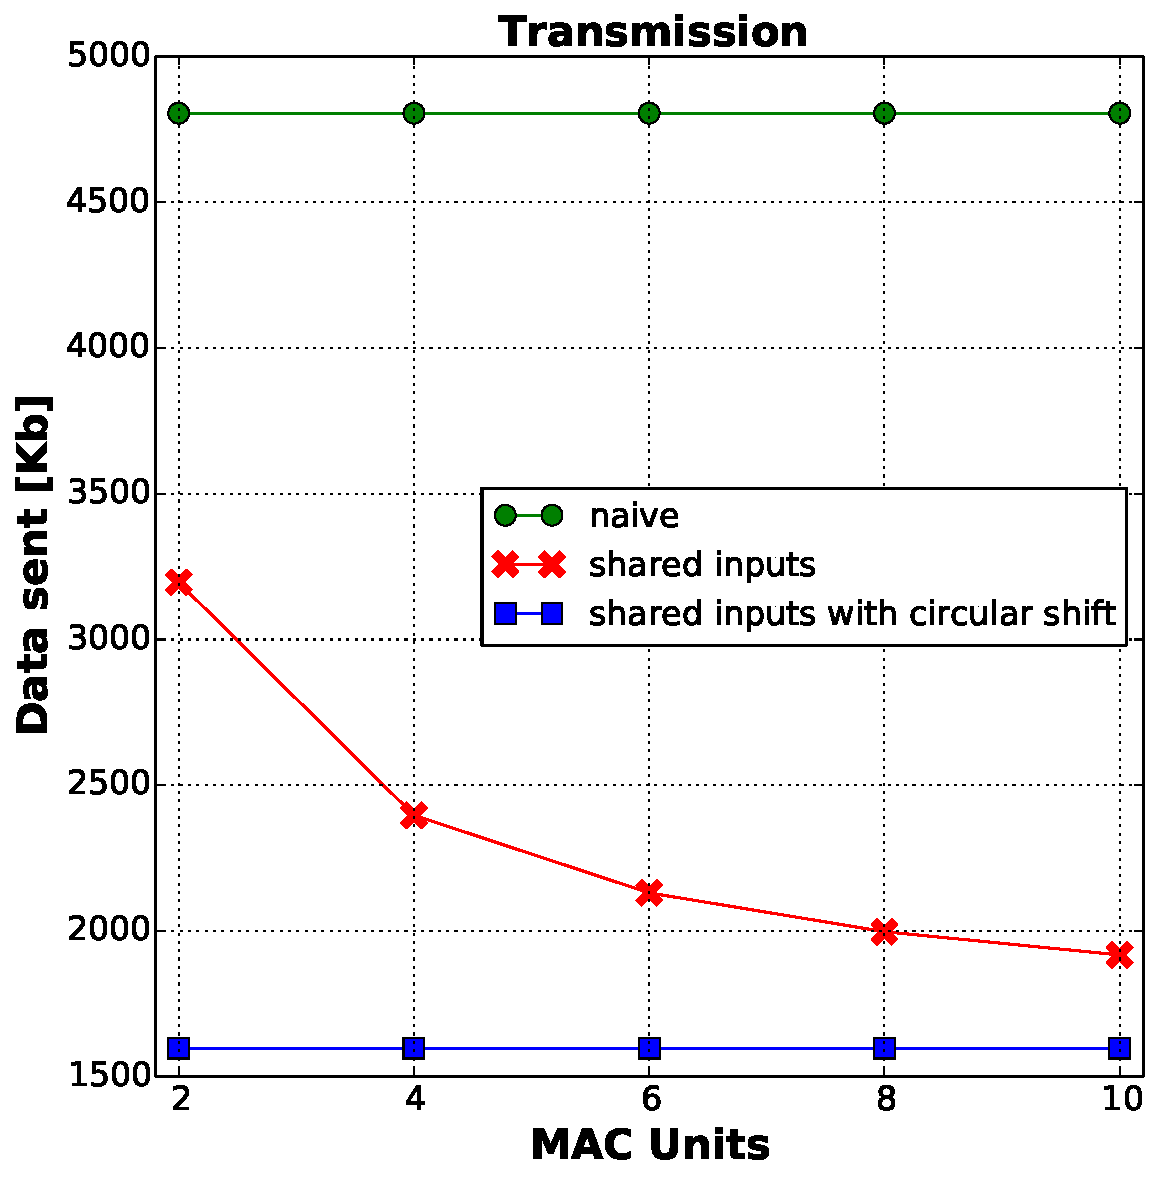
\includegraphics[scale=0.3]{data_sent}%
\label{transmitted}}
\caption{Comparación entre abordajes para una imagen de $1600\times1024$px y un kernel de $3\times3$.}\label{comp}
\end{figure}

Para asegurar un diseño escalable usando el abordaje de entradas compartidas con
desplazamiento circular, se concentró toda esta lógica en el MMU, simplificando
el diseño de los bloques restantes.

Este bloque, en cada iteración, mantiene un seguimiento de las posiciones de
memoria donde el lote entrante debe ser almacenado, la información que debe
alimentar a cada unidad MAC, las columnas de memoria donde la información
procesada debe ser almacenada y del orden en el cual la información procesada
debe ser devuelta.

Para cumplir con todas sus funciones, internamente el bloque se
compone de dos partes: una combinacional, llamada \textit{data multiplexer}, donde se
hace el encaminado de la información desde y hacia las memorias y las MACs, y
una parte secuencial basada en una máquina de estados finitos (FSM) que maneja
las señales de control de las memorias (write enable) y las señales de control
del data multiplexer.

\begin{table}
% increase table row spacing, adjust to taste
\renewcommand{\arraystretch}{1.3}
% if using array.sty, it might be a good idea to tweak the value of
% \extrarowheight as needed to properly center the text within the cells
\caption{Codificación de estados globales con las de señales SoP y EoP.}\label{MMU:glob_states}
\centering
% some packages, such as mdw tools, offer better commands for making tables
% than the plain latex2e tabular which is used here.
\begin{tabular}{|c|c|c|}
  \hline
  \textbf{Estado global} & \textbf{EoP} & \textbf{SoP}\\\hline
  Image Load             & 0            & 0           \\\hline
  Run                    & 1            & 0           \\\hline
  Out                    & 0            & 1           \\\hline
\end{tabular}           
\end{table}

El número de estados de la FSM esta dado por el número de iteraciones $It$ de la
ecuación~\ref{niter}. Cada estado de esta FSM interna representa una combinación de como se deben
escribir y leer los datos en las distintas columnas y no debe confundirse con
los estados globales del módulo explicados en la sección~\ref{states_subsecc}. Dichos
estados globales le son informados al MMU mediante dos señales de control:
comienzo de procesamiento (SoP) y fin de procesamiento (EoP). La
tabla~\ref{MMU:glob_states} muestra la codificación de dichas señales, se
observa que no están presentes todos los estados, esto es porque los estados
faltantes no afectan al comportamiento del MMU.\@ Además, el se cuenta con una
tercera señal, donde se informa que el siguiente dato debe ser escrito y leído
en la siguiente columna de memoria. 

El data multiplexer internamente se compone exclusivamente de multiplexores, que
pueden ser agrupados y clasificados en dos bloques más pequeños de acuerdo a la
función que cumplen: 

\begin{itemize}
 \item \textbf{$MMB$(Memory Multiplexer Blocks)}
  \item \textbf{$PMB$(Processing Multiplexer Blocks)}
\end{itemize}

La figura~\ref{mmu_routing} muestra el flujo de información entre unidades MAC,
MMU (data multiplexer) y las memorias. 
Los $MMB$ hacen el routing de la información sin procesar (raw data) y la
información desde las unidades $MAC$ hacia las memorias. 
Los $PMB$ hacen el routing de la información desde las memorias hacia las
unidades $MAC$. La figura~\ref{mmu_structure} muestra como están formados ambos
bloques.

\begin{figure}
\centering
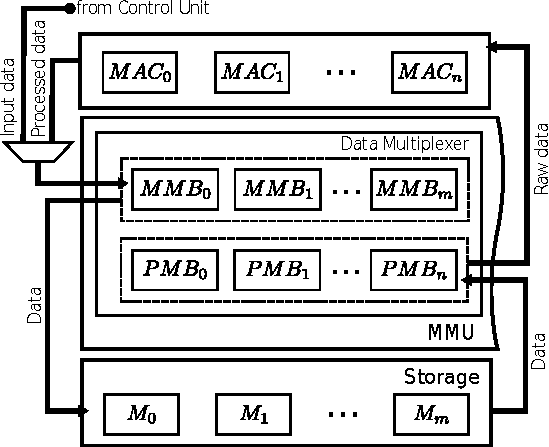
\includegraphics[scale=0.9]{muxes}
\caption{Enrutamiento de información}\label{mmu_routing}
\end{figure}

\begin{figure}
\centering
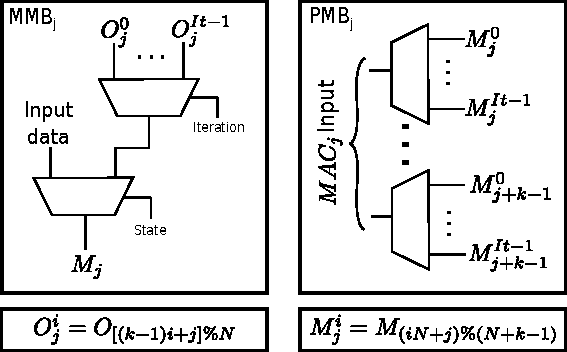
\includegraphics{muxes_cont}
\caption{Estructura de los bloques MMB y PMB.}\label{mmu_structure}
\end{figure}

Tanto los bloques $MMB$ como los $PMB$ tienen un numero de entradas proporcional
al numero de estados de la $FSM$ interna del bloque $MMU$. Las entradas
a sus multiplexores se definen respectivamente: 
\begin{equation}%\label{niter}
  O_j^i = O_{[(k-1)i+j]\%N}
\end{equation}
\begin{equation}%\label{niter}
  M_j^i = M_{(iN+j)\%(N+k-1)}
\end{equation}
donde el símbolo $ \% $ representa la operación módulo, e $i$ toma valores desde
$0$ a $It-1$.